% Created 2023-05-14 Sun 13:21
% Intended LaTeX compiler: pdflatex
\documentclass[24pt]{article}
\usepackage[utf8]{inputenc}
\usepackage[T1]{fontenc}
\usepackage{graphicx}
\usepackage{longtable}
\usepackage{wrapfig}
\usepackage{rotating}
\usepackage[normalem]{ulem}
\usepackage{amsmath}
\usepackage{amssymb}
\usepackage{capt-of}
\usepackage{hyperref}
\usepackage{minted}
\usepackage{babel}
\renewcommand*{\contentsname}{İçindekiler}
\usepackage{parskip}
\setlength{\parindent}{15pt}
\usepackage{setspace}
\onehalfspacing
\usepackage{unicode-math}
\usepackage{tikz}
\usepackage{qrcode}
\usemintedstyle{emacs}
\usepackage{geometry}
\usepackage[margin=1.0in]{geometry}
\hypersetup{colorlinks = true}
\author{---}
\date{\textit{[2023-05-15 Mon]}}
\title{Mobilen Dergi 1}
\hypersetup{
 pdfauthor={---},
 pdftitle={Mobilen Dergi 1},
 pdfkeywords={},
 pdfsubject={},
 pdfcreator={Emacs 29.0.50 (Org mode 9.6.5)}, 
 pdflang={Turkish}}
\begin{document}

\maketitle
\begin{center}

\includegraphics[width=96px]{~/me/org/roam/resources/mobilen/common/mobilen_logo.jpg}
\end{center}
\tableofcontents

\newpage
\thispagestyle{empty}

\section{iOS SwiftUI Swipe Actions}
\label{sec:orgd73e377}
\uline{\href{https://tr.linkedin.com/in/suat-karakusoglu}{Suat Karakuşoğlu} tarafından yazıldı.}

\begin{figure}[htbp]
\centering
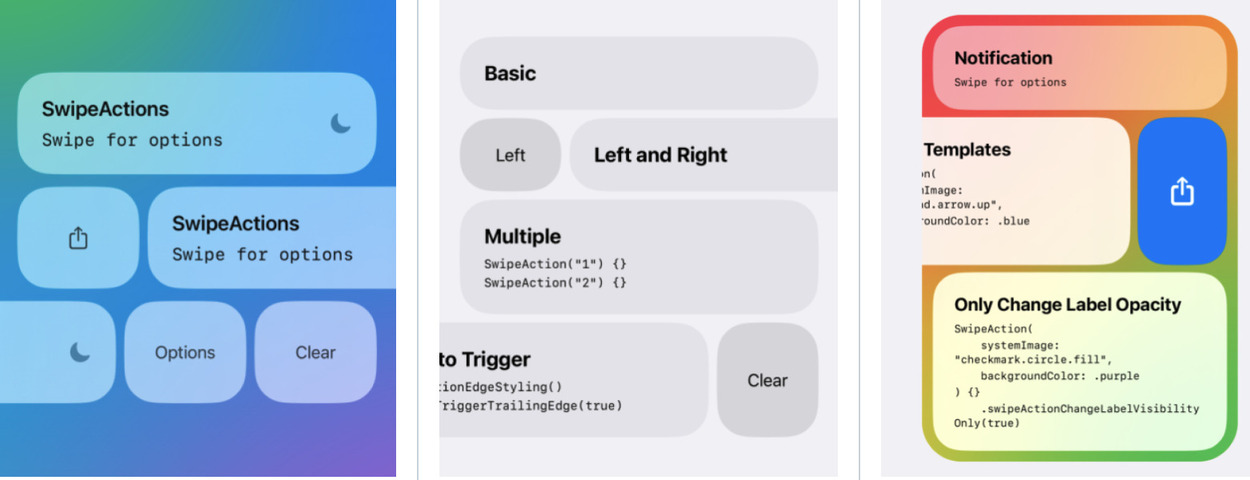
\includegraphics[width=\textwidth]{./resources/mobilen/dergi_1/SwipeActions.jpg}
\caption{Örnek Swipe Actions}
\end{figure}

\subsection{Swipe Actions nedir?}
\label{sec:org73a425e}
Merhabalar, herhangi bir ui elemanının üzerinden \texttt{swipe} ile çıkan aksiyonlar iOS kullanıcı deneyiminde önemli rol oynuyor.

Kullanıcı deneyimi açısından view'ın altında gizli, sağından veya solundan çıkan bu aksiyonlar görünmüyor olsa bile özellikle iOS kullanıcıları bu davranışı listelerde arayabiliyor.

Davranış olarak sağ ve sol demek yerine burada tercih edilen jargon \texttt{leading} ve \texttt{trailing}, bunun başlıca sebebi dillerin sağdan sola veya soldan sağa olarak 2 farklı şekilde yazılabilmesi.
Soldan sağa yazılan dillerde sol-leading, sağ trailing iken, arapça-farsça gibi dillerde sol-trailing, sağ ise leading olmakta.

Swipe aksiyonları yazabilmek için yardımcı araçlar mevcut.

\texttt{Native} olarak SwiftUI tarafından iOS 15 ile SwiftUI List'elerine eklendi.
\href{https://developer.apple.com/documentation/swiftui/view/swipeactions(edge:allowsfullswipe:content:)}{iOS 15 SwiftUI SwipeActions} adresinden native yöntem incelenebilir.

Ancak iOS-14 destekliyorsanız veya herhangi bir SwiftUI view'e swipe aksiyonları eklemek isterseniz bunun için güzel bir SwiftUI component'i açık kaynak olarak geliştirilip github'a \texttt{spm} destekli olarak koyulmuş.

Bu yazımızda \href{https://github.com/aheze/SwipeActions}{Açık Kaynak SwipeActions Reposu}'nu inceleyeceğiz.

\subsection{SwipeActions Kullanımı}
\label{sec:org279bf97}

\begin{listing}[htbp]
\begin{minted}[,frame=lines]{swift}
import SwiftUI
import SwipeActions

struct ContentView: View {
    var body: some View {
        SwipeView {
            Text("Hello")
              .frame(maxWidth: .infinity)
              .padding(.vertical, 32)
              .background(Color.blue.opacity(0.1))
              .cornerRadius(32)
        } trailingActions: { _ in
            SwipeAction("World") {
                print("Tapped!")
            }
        }
          .padding()
    }
}
\end{minted}
\caption{Örnek bir swipe aksiyon eklemesi}
\end{listing}

\subsection{Kaynak Kod Okuma: \texttt{PreferenceKey} kullanımı}
\label{sec:orgb6a5470}
Veri iletişimi view componentleri arasında Environment Objeler uzerinden \texttt{Parent} → \texttt{Child} view yönünde olabiliyor.
Veya data binding ile \texttt{@Binding} çift taraflı \texttt{reactive} şekilde sağlanabiliyor.

PreferenceKey ile olan bu veri iletişiminde ise diğer bir ihtiyaç olan ise \texttt{child} → \texttt{parent} arasında veri geçişi yapabiliyoruz.

\begin{listing}[htbp]
\begin{minted}[,frame=lines]{swift}
struct AllowSwipeToTriggerKey: PreferenceKey {
    static var defaultValue: Bool? = nil
    static func reduce(value: inout Bool?, nextValue: () -> Bool?)
    { value = nextValue() }
}
\end{minted}
\caption{Preference Key tanımlama}
\end{listing}

Preference key tanımlarken ihtiyaç duyulan \texttt{PreferenceKey} protocol'unu \texttt{conform} etmek.
Bunun için bir varsayılan değer \texttt{defaultValue} gerekiyor.
Ayrıca ikinci olarak \texttt{reduce} fonksiyonu, bu fonksiyon dışarıdan sağlanan değerin preference olarak set edilmesine müdahale edilebilecek noktayı sağlıyor.

Kullanımı için 2 tane \texttt{modifier}'imiz mevcut: \texttt{preference} ve \texttt{onPreferenceChange}.

\begin{listing}[htbp]
\begin{minted}[,frame=lines]{swift}
view.preference(key: AllowSwipeToTriggerKey.self, value: allowSwipeToTrigger)
\end{minted}
\caption{Preference Key ile veriyi yukarı aktarma}
\end{listing}

\begin{listing}[htbp]
\begin{minted}[,frame=lines]{swift}
view.onPreferenceChange(AllowSwipeToTriggerKey.self) { allow in
    /// Unwrap the value first (if it's not the edge action, `allow` is `nil`).
    if let allow {
        swipeToTriggerLeadingEdge = allow
    }
}
\end{minted}
\caption{Preference Key ile aşağıdan gelen veriyi okuma}
\end{listing}

Ayrıca apple sdk'inde de \texttt{navigationTitle} modifier'i ile \texttt{preference key} kullanılarak \texttt{child} üzerinden çağırılan bir method ile üst view'deki \texttt{title}'i değiştirebiliyor.

Özetle hiyerarşide yukarı veri taşıyabilmek için kullanılan bu yapının kullanıldığını görüyoruz.
Daha detaylı anlamak için \href{https://swiftwithmajid.com/2020/01/15/the-magic-of-view-preferences-in-swiftui/}{Magic of View Preferences in SwiftUI} yazısına göz atabilirsiniz.

\subsection{Referanslar}
\label{sec:org6710808}
\begin{enumerate}
\item \href{https://developer.apple.com/documentation/swiftui/preferences?changes=\_7}{Apple PreferenceKey Dokümantasyonu}
\item \href{https://swiftwithmajid.com/2020/01/15/the-magic-of-view-preferences-in-swiftui/}{Magic of View Preferences in SwiftUI}
\end{enumerate}

\newpage
\thispagestyle{empty}

\section{Netfox ile iOS uygulamalarda network izlemek}
\label{sec:org3089b19}
\uline{\href{https://www.linkedin.com/in/ugurcan-durak/}{Uğurcan Durak} tarafından yazıldı.}

\begin{figure}[htbp]
\centering
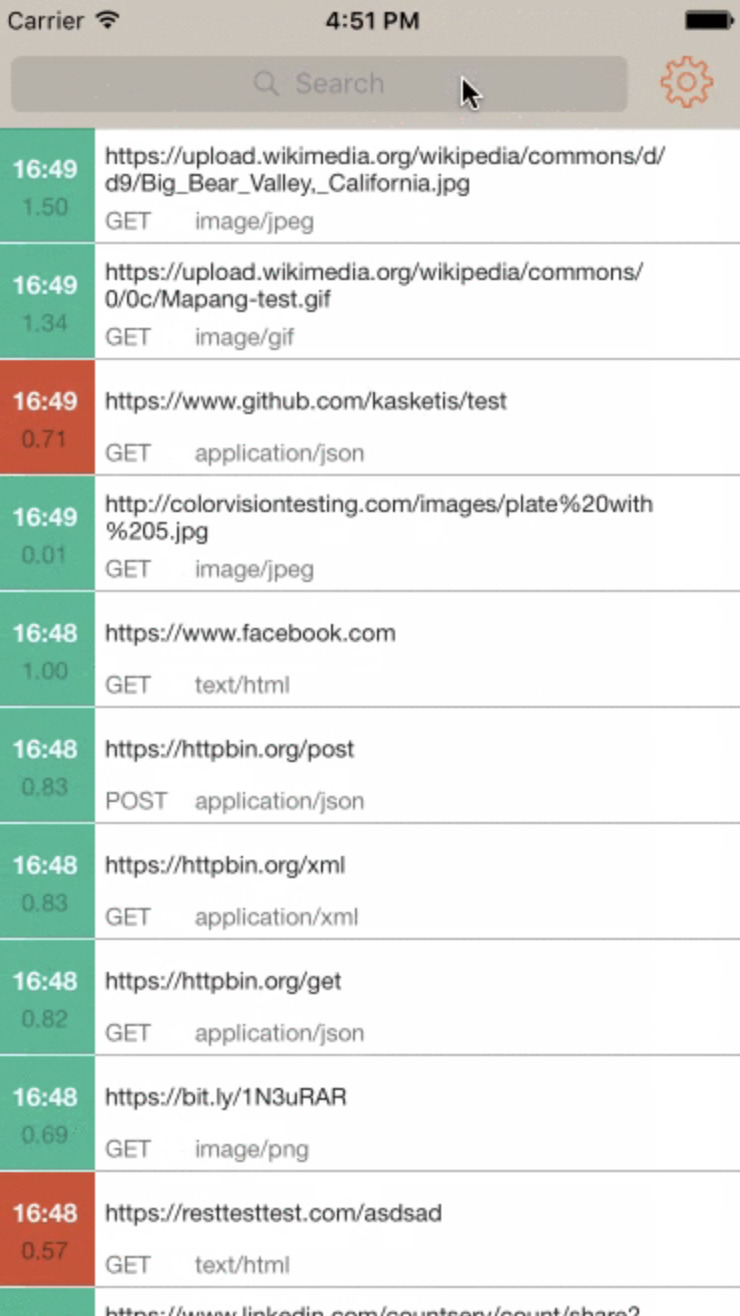
\includegraphics[width=200px]{./resources/mobilen/dergi_1/NetFoxImage.jpg}
\caption{\href{https://raw.githubusercontent.com/kasketis/netfox/master/assets/overview1\_5\_3.gif}{Netfox'u İzlemek için tıkla}}
\end{figure}

Merhabalar, bu yazıda mobil cihazda network isteklerini detaylı şekilde görüntülemek için kullanılan faydalı olduğunu düşündüğüm \textbf{\href{https://github.com/kasketis/netfox}{Netfox}} kütüphanesinden bahsedicem.

Çok detaya girmeden genel hatlarıyla nedir? nasıl kullanılır? gibi başlıklarla değineceğim. Hadi başlayalım :)

\subsection{Netfox Nedir?}
\label{sec:orgb09c0b9}
\textbf{\href{https://github.com/kasketis/netfox}{Netfox}} kütüphanesi, tüm network işlemlerini mobil cihaz üzerinden detaylı bir şekilde görüntüleyebileceğimiz \texttt{open source} bir kütüphanedir.

Netfox'u uygulama içerisinde istediğimiz bir anda başlatıp anlık olarak uygulamamızın yapmış olduğu tüm istekleri listeleyebilir ve detaylı bir şekilde \texttt{body}, \texttt{header}, \texttt{response} gibi tüm network etkileşimlerini inceleyebiliriz.

Bu tarz kütüphanelerin en güzel yanı, mobil cihazımız bilgisayara bağlı olmadan da istediğimiz bir anda network log'larına bakabiliyor olmamızdır. Bu özellik testçiler için oldukça faydalıdır çünkü herhangi bir hata anında doğrudan developer'a bildirmek yerine log'ları inceleyip hata hakkında fikir sahibi olabilirler.

\subsection{Netfox Nasıl Kullanılır?}
\label{sec:org05162ee}
Netflox'ın kullanımı ve projeye entegre edilmesi oldukça basittir.

Varsayılan davranışı \textbf{\textbf{shake}} olarak belirlenmiş olsada custom bir şekilde istediğimiz bir butona ya da bir view event'ine atayarak Netfox'ı başlatabiliriz. Öncelikle projeye nasıl eklenir ona bakalım.

\subsection{Netfox'un Projeye Eklenmesi}
\label{sec:org1c66089}
\begin{enumerate}
\item Netflox kütüphanesini \textbf{\textbf{SPM}}, \textbf{\textbf{CocoaPods}} ve \textbf{\textbf{Carthage}} olmak üzere üç ayrı yöntem ile projemize ekleyebiliriz. Bu yöntemlerden herhangi biriyle eklediğinizi varsayarak bir sonraki adıma geçiyorum.

\item Kütüphaneyi projeye ekledik şimdi ise initiliaze edeceğiz. Bunun için AppDelegate class'ına gidip aşağıdaki gibi gerekli kodları ekliyoruz.
\end{enumerate}

\begin{listing}[htbp]
\begin{minted}[,frame=lines]{swift}
#if DEBUG
import netfox
#endif
\end{minted}
\caption{Netfox Import}
\end{listing}

Burada  \textbf{\textbf{\#if DEBUG}} ve \textbf{\textbf{\#endif}} kodlarını ekleyerek kodun sadece debug moddayken import olmasını sağlıyoruz. Daha sonra uygulama ilk başlatıldığında hazır hale gelmesini istediğim için aşağıdaki gibi başlatıcı fonksiyonun içerisine kodlarımızı ekliyoruz.

\begin{listing}[htbp]
\begin{minted}[,frame=lines]{swift}
func application(
  _ application: UIApplication,
  didFinishLaunchingWithOptions launchOptions: [UIApplication.LaunchOptionsKey: Any]?
) -> Bool {
    #if DEBUG
    NFX.sharedInstance().start()
    NFX.sharedInstance().setGesture(.shake)
    #endif
}
\end{minted}
\caption{Netfox başlatma}
\end{listing}

Burada \textbf{\textbf{start()}} methodunu çağırarak Netfox'ı initiliaze ediyoruz ardından \textbf{\textbf{setGesture()}} ile Netfox'ın nasıl açılacağını belirliyoruz.

Varsayılan davranışı shake olduğundan özellikle belirtmenize gerek yok örnek olması açısından ekledim. Siz dilerseniz \textbf{\textbf{custom}} parametresini geçip daha sonra dilediğiniz yerde \textbf{\textbf{show()}} methodu ile açılmasını sağlayabilirsiniz.

\subsection{Netfox Özetle}
\label{sec:orgae9b24e}
Evet hepsi bu kadar :) Şimdi dilediğiniz gibi cihazı sallayarak ya da atamış olduğunuz bir buton ile Netfox'ı başlatabilir ve log'ları inceleyebilirsiniz.

Daha detaylı incelemek isteyenler için aşağıya link bırakıyorum. Umarım faydalı olur zaman ayırdığınız için teşekkürler.

\subsection{Referanslar}
\label{sec:org2d8949f}
\begin{enumerate}
\item \href{https://github.com/kasketis/netfox}{Netfox Github Kütüphanesi}
\item \href{https://raw.githubusercontent.com/kasketis/netfox/master/assets/overview1\_5\_3.gif}{Örnek Kullanım Vidyosu}
\end{enumerate}

\newpage
\thispagestyle{empty}

\section{XCode Breakpoints}
\label{sec:org987cf70}
\uline{\href{https://tr.linkedin.com/in/alper-cem-\%C3\%B6zt\%C3\%BCrk-a625671a8}{Alper Cem Öztürk} tarafından yazıldı.}
\end{document}